\section{Einführung in die Logistik und SCM}

\textbf{Logistik}:
\begin{itemize}
	\item \textbf{Definition}: 
	\begin{itemize}
		\item Planung, Implementierung und Kontrolle 
		\item von effizienten, effektiven Vor- und Rückflüssen 
		\item sowie der Lagerung von Gütern, Dienstleistungen und Informationen 
		\item zwischen Ursprungs- und Verbrauchsort 
		\item mit dem Ziel, die Kundenanforderungen zu erfüllen
	\end{itemize}
	\item \textbf{Aufgabe der Logistik} ist es,
	\begin{itemize}
		\item den Kunden mit dem richtigen Produkt, am richtigen Ort, zur richtigen Zeit,
		\item unter gleichzeitiger Optimierung eines vorgegebenen Leistungskriteriums (z. B.
		Minimierung der Gesamtkosten),
		\item und unter Berücksichtigung gegebener Anforderungen (z. B. Servicegrad) und
		Beschränkungen (z. B. Budget) zu versorgen
	\end{itemize}
	\item \textbf{7 R's der Logistik}:
	\begin{itemize}
		\item Richtiges Produkt
		\item Richtige Zeit
		\item Richtiger Ort
		\item Richtige Menge
		\item Richtige Qualität
		\item Richtige Kosten
		\item Richtige Information
	\end{itemize}
	\item \textbf{Auf was bezieht sich Logistik heute?}
	\begin{itemize}
		\item Alle arbeitsteiligen Wirtschaftssysteme, in denen es auf zeit-, kosten- und mengenabhängige Verteilung von Gütern und Dienstleistungen ankommt
	\end{itemize}
\end{itemize}
\bigskip
\textbf{Supply Chain}: 
\begin{itemize}
	\item Komplexes, unternehmensübergreifendes, interlogistisches System, das die Vorgänge und Funktionen der Beschaffung, Produktion, Verarbeitung, Lagerung und Distribution von Objekten umfasst
	\item Keine einfache Kette, sondern ein komplexes Netzwerk mit sich verzweigenden und zusammenführenden Informations- und Materialflüssen
\end{itemize}

\textbf{Supply Chain Management (SCM)}:
\begin{itemize}
	\item Koordination und Kollaboration von Stakeholdern entlang der gesamten Supply Chain, d.h. auch über die eigene Organisation hinaus, insbesondere mit Zulieferern, Zwischenhändlern, Service-Dienstleistern und Kunden
	\item Umfasst alle Aktivitäten des Logistik Management sowie Produktionsaktivitäten, Vertrieb, Produktdesign, Finanzen und IT
\end{itemize}
\bigskip
\textbf{Supply Chain Network}:
\begin{center}
	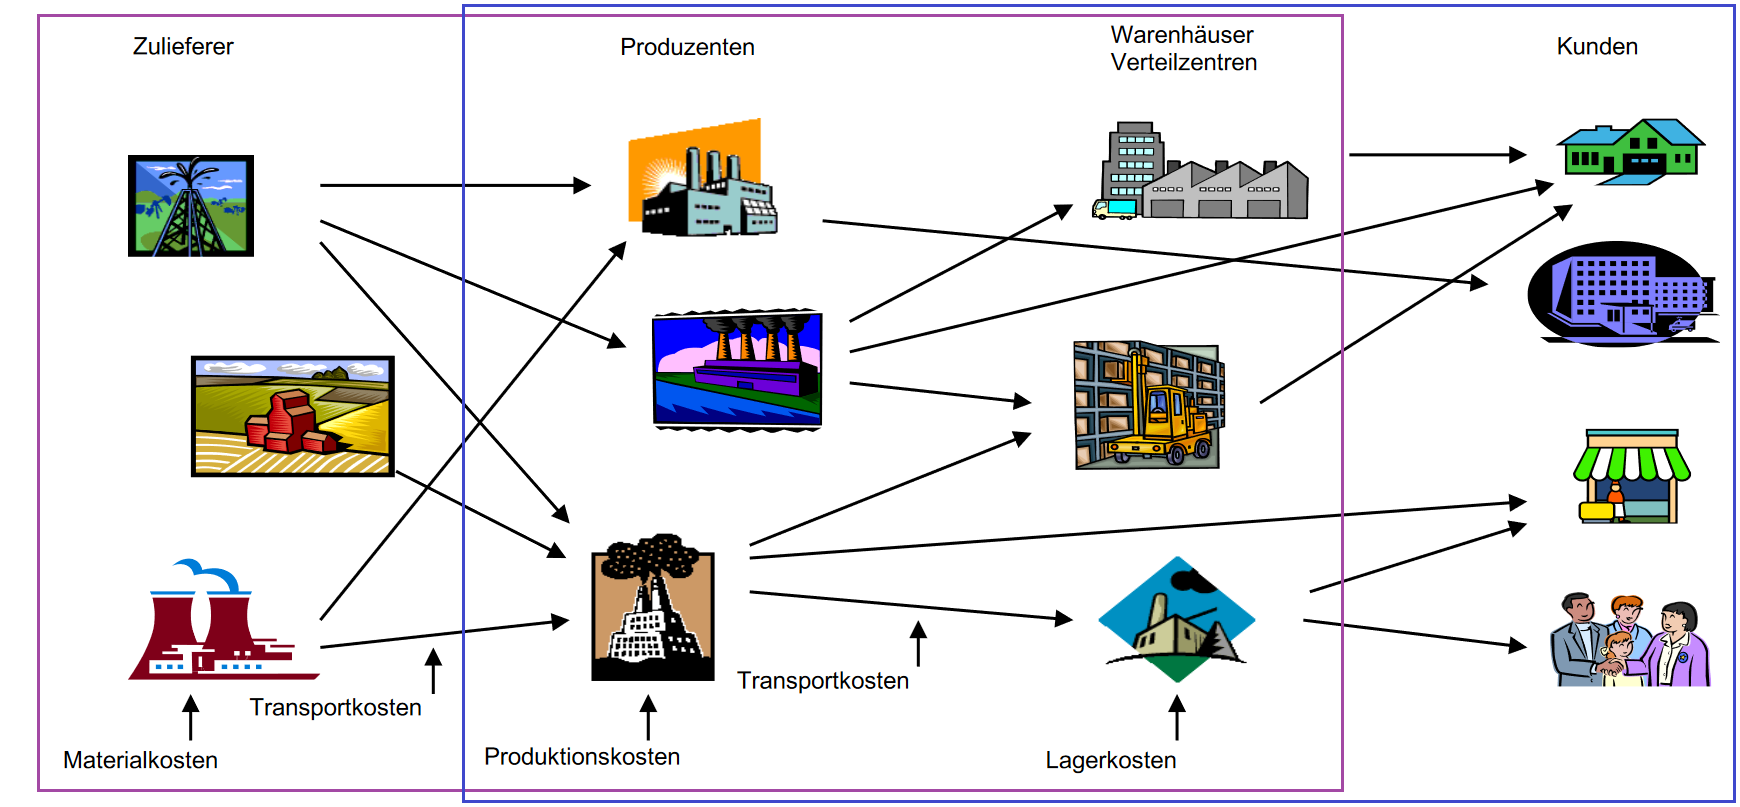
\includegraphics[width=\textwidth]{images/scn.png}
\end{center}
\begin{itemize}
	\item \textcolor{violet}{Quellen}, Lieferanten, Auslieferer stellen Objekte zur Verfügung, z.B. Rohstofflager, Produktionsanlagen, Fabriken, Vorratslager, Importlager, Logistikzentren
	\item \textcolor{blue}{Senken} oder Anlieferstellen haben Nachfragen nach Objekten, z.B. Einzelhändler, Märkte, Filialen, Konsumenten, Müllverbrennungsanlagen
	\item Warenquellen können selbst Empfänger von Gütern aus anderen Quellen sein
	\item Handel und Konsumenten sind wiederum Quellen von Leergut, Restoffen und Verpackungsabfall, die entsorgt werden müssen
	$\rightarrow$ \textbf{Reverse Logistics}
\end{itemize}
\bigskip
\textbf{Planungsebenen des Supply Chain Managements}:
\begin{itemize}
	\item \textbf{Strategisch – Supply Chain Configuration:}
	\begin{itemize}
		\item Entscheidungen mit langfristigem Effekt und hohem Kapitalaufwand
		\item Planungszeitraum: mehrere Jahre
		\item Daten: aggregiert, basieren auf Vorhersagen, oft unvollständig oder ungenau
		\item \textbf{Beispiele}: Anzahl, Standorte und Kapazitäten von Einrichtungen, Investitionen in Produktions- und Lageranlagen, Layout von Einrichtungen
	\end{itemize}
	\item \textbf{Taktisch – Supply Chain Planning:}
	\begin{itemize}
		\item Entscheidungen, die die effektive Allokation von Produktions- und
		Distributionsressourcen betreffen
		\item Planungszeitraum: 3 Monate bis 1 Jahr
		\item Daten: detailliert, basieren auf Vorhersagen
		\item \textbf{Beispiele}: Beschaffungs- und Produktionsentscheidungen, Wahl von Transport- und Versandstrategien, Lagerbestandsplanung
	\end{itemize}
	\item \textbf{Operativ – Supply Chain Execution:}
	\begin{itemize}
		\item Erstellt zeit- und mengengenaue unmittelbar umsetzbare Vorgaben
		für die Ausführung der Prozesse
		\item Planungszeitraum: täglich, wöchentlich
		\item Daten: sehr konkret, detailliert, bis auf unvorhergesehene Störungen
		vollständig aus ERP System bekannt
		\item \textbf{Beispiele}: Scheduling (Produktion), Zuweisung von Aufträgen zu Maschinen, Auftragsverarbeitung, Fahrzeug-Routing, LKW-Beladung
	\end{itemize}
\end{itemize}
\begin{figure}[h]
\begin{center}
	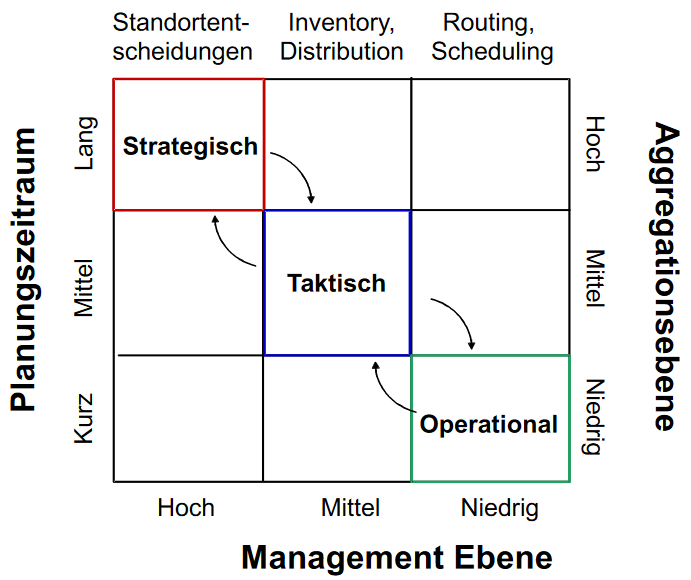
\includegraphics[width=0.5\textwidth]{images/scm-ebenen.png}
	\caption*{Aggregationsebene: Wie detailliert sind die Daten}
\end{center}
\end{figure}

\textbf{Logistik vs. SCM}:
\begin{itemize}
	\item \textbf{Logistik}: Betrachtung der Material- und Erzeugnisflüsse unter Berücksichtigung von Informations- und Wertströmen \underline{innerhalb der eigenen Organisation}
	\item \textbf{SCM}: Gesamtes logistisches Wertschöpfungsnetz mit Lieferanten, Produzenten, Händlern, Konsumenten 
	
	Koordination und Kollaboration von Stakeholdern entlang der gesamten Supply Chain, auch \underline{über die eigene Organisation hinaus}
\end{itemize}

\textbf{Operations Research:}
\begin{itemize}
	\item Analysiert praxisnahe, komplexe Problemstellungen, um möglichst gute Entscheidungen zu treffen
	\item Probleme werden mithilfe mathematischer Modelle formuliert und mit mathematischen Lösungsmethoden gelöst
	\item Anwendbar auf verschiedenste Probleme in Logistik und SCM
\end{itemize}
\bigskip
\textbf{Vorgehen beim Lösen von Problemen mit OR:}
\begin{itemize}
	\item Überführe realwirtschaftliches Logistikproblem in abstraktes, logistisches Modell
	\item Wandle logistisches Modell in OR-Modell (LP/MILP/MIP) um und löse mit bekannten Werkzeugen
	\item Interpretation der OR-Modell-Lösung und Schlussfolgerung für das reale
	Problem
\end{itemize}
\begin{center}
	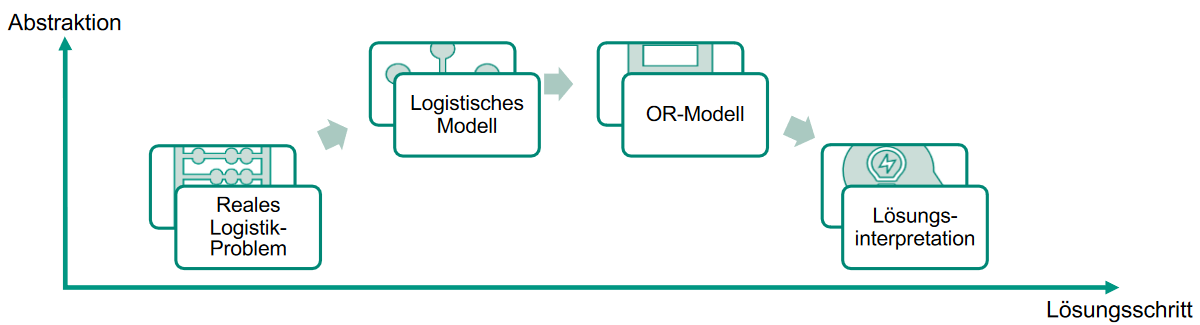
\includegraphics[width=0.8\textwidth]{images/or-workflow.png}
\end{center}
\begin{itemize}
	 \item \textit{Beispiel siehe Logistik VL 1, F27-34}
	 \item \textit{Rechenbeispiele siehe Logistik Tutblatt 1}
\end{itemize}
\bigskip
\textbf{Wichtige Software für die Logistik:}
\begin{itemize}
	\item \textbf{Enterprise Resource Planning Systeme (ERP)} erfassen Daten aller wesentlichen Geschäftsfunktionen (z.B. Buchhaltung, Personalwesen) konsistent und up-to-date und machen diese unternehmensweit verfügbar (z.B. SAP, Oracle)
	\item Erweiterung zu \textbf{Advanced Planning Systems (APS)} helfen, komplexe Planungsaufgaben im SCM zu erfüllen und rationale Entscheidungen zu unterstützen
	\item APS nehmen die im ERP-System erhobenen Daten in Modelle entgegen und lösen die so entstandenen Probleme mittels OR-Algorithmen
\end{itemize}